\documentclass[noend]{amsproc}

\renewcommand{\arraystretch}{1.3}

\usepackage{amsthm,amsmath,amsfonts,mathrsfs,amssymb}
\usepackage{algorithm}
\usepackage{algorithmicx, algpseudocode}
\usepackage[T1]{fontenc}   % for bold \Singular
\usepackage{multirow}
\usepackage{natbib}
\usepackage{tikz}
\usetikzlibrary{matrix,arrows}

\newtheorem{theorem}{Theorem}
\newtheorem{defn}[theorem]{Definition}
\newtheorem{prop}[theorem]{Proposition}
\newtheorem{lemma}[theorem]{Lemma}
\theoremstyle{definition}
\newtheorem{remark}[theorem]{Remark}

% ALGORITHM style
\renewcommand{\algorithmicrequire}{\textbf{Input:}}
\renewcommand{\algorithmicensure}{\textbf{Output:}}
\newcommand{\algorithmicbreak}{\textbf{break}}
\newcommand{\Break}{\State \algorithmicbreak}
\renewcommand{\algorithmicreturn}{\State \textbf{return}}
\renewcommand{\Re}{\operatorname{Re}}
\renewcommand{\Im}{\operatorname{Im}}
\newcommand{\Singular}{\textsc{Singular}}
\newcommand{\realclassify}{\texttt{realclassify.lib}}
\newcommand{\classify}{\texttt{classify.lib}}


\DeclareMathOperator{\ord}{ord}
\DeclareMathOperator{\requiv}{\overset{r}{\sim}}
\DeclareMathOperator{\m}{\mathfrak{m}}
\DeclareMathOperator{\jet}{jet}
\DeclareMathOperator{\corank}{corank}
\DeclareMathOperator{\supp}{supp}
\DeclareMathOperator{\sign}{sign}
\DeclareMathOperator{\diag}{diag}
\DeclareMathOperator{\NF}{NF}
\DeclareMathOperator{\N}{\mathbb{N}}
\DeclareMathOperator{\Q}{\mathbb{Q}}
\DeclareMathOperator{\R}{\mathbb{R}}
\DeclareMathOperator{\C}{\mathbb{C}}
\DeclareMathOperator{\A}{\mathbb{A}}
\DeclareMathOperator{\Pj}{\mathbb{P}}
\DeclareMathOperator{\boldzero}{\mathbf{0}}
\DeclareMathOperator{\dash}{\textnormal{-}}

\begin{document}
\section{The Equivalence Classes of the Exceptional Singularities and the singularities of main type $J_{10+k}$}

Throughout this section we choose a weight $w$ (or weights) on the variables in $\R[[x_1,\ldots,x_n]]$ and in $\C[[x_1,\ldots,x_n]]$ such that the weighted degree of $x_i$, $w\dash\deg(x_i),\ \forall i$ are natural numbers. For $f,g\in\R[[x_1,\ldots,x_n]]$ or $f,g\in\C[[x_1,\ldots,x_n]]$ we mean by $f*_wg$, $w\dash\deg(f)* w\dash\deg(g)$, where $*$ is any one of $<,\le,>,\ge,=$. We denote the weighted $j\dash\jet$ of a power series $f$ by $j\dash w\dash\jet(f)$.

For background regarding the following definitions and results we refer to \cite{A1974}.

\begin{defn}
A power series (polynomial, germ, function) has filtration $d$ if all its monomials are of weighted degree $d$ or higher. The power series (polynomials, germs, functions) of filtration $d$ form a linear space $E_d^w$.
\end{defn}

Note that $E_{d'}^w\subseteq E_d^w$ if $d<d'$. Since the filtration of a product, $E_{d'}^w\cdot E_d^w$, is the sum of the filtrations of the factors, $d'+d$, it follows that $E_d^w$ is an ideal in the ring of power series (polynomials, germs, functions). We denote the ideal of $E_d^w$ consisting of series of filtration strictly greater than $d$ by $E_{>d}^w$. If the weight of all the variables are $1$ we only write $E_d$. 

\begin{defn}\label{phi}
Let $\phi$ be an $\R$-algebra or $\C$-algebra automorphism of $\R[[x_1,\ldots,x_n]]$ or $\C[[x_1,\ldots,x_n]]$  and let $w$ be a chosen weight on the variables. 
\begin{itemize}
\item[(i)] For $j > 0$ we define the
\emph{$j$-$w$-jet} of $\phi$, denoted by $\phi_j^w$, to be the automorphism given by
\[
\phi_j^w(x_i) := w\dash\jet(\phi(x_i),w\dash\deg(x_i)+j) \quad \forall i = 1,\ldots,n \,.
\]
If the weight of all the variables are $1$, we only write $\phi_j$.\\
\item[(ii)] $\phi$ has filtration $d$ if,  $\forall\lambda$,
\[(\phi-1)E_\lambda^w\subset E_{\lambda+d}^w.\]
\end{itemize}
\end{defn}

Note that $\phi_0(x_i)=\jet(\phi(x_i),1)\ \forall i$. Furthermore note that $\phi_0^w$ has filtration $\le 0$ and, for $j>0$, if $\phi_{j-1}^w=1$, then $\phi_j^w$ has filtration $j$. 


The infinitesimal analogue of Definition \ref{phi}(ii) is:

\begin{defn}
A formal vector field $v=\sum_i v_i\frac{\partial}{\partial x_i}$ has filtration $d$ if the directional derivitive raises the filtration by not less than $d$, i.e.~$L_vE^w_\lambda\subset E^w_{\lambda+d}$, where $L_v(f)=\sum_i v_i\frac{\partial f}{\partial x_i}$.
\end{defn}

The following result is proven in \cite{A1974} (Corollary 6.7).

\begin{lemma}\label{vectorlemma}
Let $f=f_0+f_1+f_2$, where $f_0\in E^w_d$, $f_1\in E^w_{>d}$ and $f_2\in E^w_{d+\delta}$, and let $\phi$ be an automorphism defined by $\phi(x_i)=x_i+v_{0,i}+v_{1,i}$, where $v_0=\sum_iv_{0,i}\frac{\partial}{\partial x_i}$ has filtration $\delta$ and $v_1=\sum_iv_{1,i}\frac{\partial}{\partial x_i}$ has filtration strictly greater than $\delta$ where $\delta>0$. Then
\[\phi(f)=f_0+\left[ f_1+\sum_iv_{0,i}\frac{\partial f_0}{\partial x_i}\right]+R,\]
where $R\in E^w_{>d+\delta}$.
\end{lemma}

\begin{prop}
Considering the real exceptional cases of corank 2, allowing only real transformations, there are no equivalences that hold between different subcases and different chosen values of the parameter $a$.
\end{prop}

\begin{proof}
Recall that a normal form is a family of polynomials. Let $f$ be an arbitrary polynomial in any one of the exceptional normal forms. Now, $f$ can be written as $f=f_0+f_1$, where $f_0$ is the sum of the terms not having the chosen value of the parameter as coefficient and $f_1$ is the term that has the coefficient as parameter. We choose a weighted degree $w$, with the weights of $x$ and $y$ natural numbers, such that the terms in $f_0$ have the same degree $w_0$. Hence $f_0$ is the quasihomogeneous part of $f$.

Let $\phi$ be an $\R$-algebra automorphism that transform $f$ to a polynomial in the same main singularity type.

Note that in the cases (a) $Z_{11}, Z_{12}, Z_{13}$:
\begin{equation}\label{a}
x^2>_w xy>_w y^2>_w x>_w y
\end{equation} 
and in the cases (b)  $W_{12}, W_{13}$:
\begin{equation}\label{b}
y^3>_wx^2>_w xy>_w y^2>_w x>_w y
\end{equation} 
and in the cases (c) $E_{12}, E_{13}, E_{14}$:
\begin{equation}\label{c}
x^2>_w xy >_w y^3>_w x>_w y^2>_w y.
\end{equation}
Let $k_0$ be the lowest jet of $f$, i.e.~$\jet(f,k_0-1)=0$ and $\jet(f,k_0)\neq 0$. Since 
\begin{eqnarray*}
\phi(f) &=& \phi_0(\jet(f,k_0))+\phi_0(f-\jet(f,k_0))+\phi^*(f)\nonumber\\
 &=& \phi_0(\jet(f,k_0))+R,\label{lowestjet}
\end{eqnarray*}
where $\phi^*=\phi-\phi_0$ and $R\in E_{>k_0}$, it is clear that
\begin{equation}\label{transxy}
\jet(\phi(x),1)=\alpha x\quad\textnormal{and}\quad\jet(\phi(y),1)=\beta y,\quad 0\neq\alpha,\beta\in\R,
\end{equation}
in the cases $Z_{11}, Z_{12}$ and $Z_{13}$ and that
\begin{equation}
\jet(\phi(x),1)=\alpha x,\quad 0\neq\alpha\in\R.\label{transx}
\end{equation}
in the other cases.

Considering the cases in (a), taking  (\ref{a}) into account, it follows that
\begin{equation*}
\frac{\partial f_0}{\partial y}y^2 =_w \frac{\partial f_0}{\partial x}xy>_w f_1\quad\textnormal{and}\quad \frac{\partial f_0}{\partial y}y^2>_w \frac{\partial f_0}{\partial x}y^2>_w f_0.
\end{equation*}
Now, $\phi=\phi''\circ\phi'$, where $\phi'$ and $\phi''$ are, respectively, defined by
\[\phi'(x)=\alpha x,\quad \phi'(y)=\beta y, \quad \phi''(x)=\frac{1}{\alpha}\phi(x), \quad\phi''(y)=\frac{1}{\beta}\phi(y).\]
If $\alpha,\beta\neq 1$, we replace $f$ by $\phi'(f)$ and $\phi$ by $\phi''$ for the next argument, showing that the coefficient of $y^2$ in $\phi(x)$ is nonzero or equivalently that the coefficient of $y^2$ in $\phi''(x)$ is nonzero.
Since the filtration of $\phi$ is positive, it follows from Lemma \ref{vectorlemma} that
\begin{equation*}
\phi(f) = f_0+c\cdot c_0\frac{\partial f_0}{\partial x}y^2+f_1+R,\quad R\in E^w_{>w\dash\deg(f_1)},
\end{equation*}
where $\phi(x) = x+cy^2+R'$, $R'\in E^w_{>w\dash\deg(y^2)}$ and $c_0,c\in\R$.
Since $\gamma_0\frac{\partial f_0}{\partial x}y^2+\gamma_1f_1\neq \gamma_2f_1$, for any $\gamma_0,\gamma_1,\gamma_2\in\R$, $\gamma_0\neq 0$, in all three cases in (a) it follows that $c=0$. Since we have assumed that $\phi(f)$ transforms $f$ to a polynomial in the same main singularity type and $\phi-\phi_0^w$ only contributes to terms in $R$, it is enough to consider $\phi_0^w$. We therefore only need to consider automorphisms $\phi$ defined by 
\begin{equation}\label{trans1}
\phi(x)=\alpha x\quad\textnormal{and}\quad\phi(y)=\beta y,\quad0\neq\alpha,\beta\in\R.
\end{equation}
Similarly, for the cases in (b), taking \ref{b} into account, we have that
\begin{equation*}
\frac{\partial f_0}{\partial y}y^2 =_w \frac{\partial f_0}{\partial x}xy>_w f_1\quad\textnormal{and}\quad \frac{\partial f_0}{\partial x}y^2>_w \frac{\partial f_0}{\partial y}x>_w f_0.
\end{equation*}
Again, if $\alpha,\beta\neq 1$ we replace $f$ by $\phi'(f)$ and $\phi$ by $\phi''$ to show that the coefficient of $x$ in $\phi(y)$ is zero or equivalently that the coefficient of $x$ in $\phi''(y)$ is zero. Since the filtration of $\phi$ is positive, it follows from Lemma \ref{vectorlemma} that
\begin{equation*}
\phi(f) = f_0+c\cdot c_1\frac{\partial f_0}{\partial y}x+c_2\cdot c_3\frac{\partial f_0}{\partial x}y^2+f_1+R,\quad R\in E^w_{>w\dash\deg(f_1)},
\end{equation*}
where $\phi(y) = y+cx+c_2y^2+R'$, $R'\in E^w_{>w\dash\deg(y^2)}$ and $c,c_1\ldots,c_3\in\R$.
Since $\gamma_0\frac{\partial f_0}{\partial y}x+\gamma_1\frac{\partial f_0}{\partial x}y^2+\gamma_2f_1\neq \gamma_3f_1$, for any $\gamma_0,\ldots,\gamma_3\in\R$,  not both $\gamma_0$ and $\gamma_1$ zero, in both cases in (b), we only need to consider automorphisms $\phi$ defined by 
\begin{equation}\label{trans2}
\phi(x)=\alpha x\quad\textnormal{and}\quad\phi(y)=\beta(y),\quad0\neq\alpha,\beta\in\R.
\end{equation}
We now consider the cases in (c). Similarly as above, we replace $f$ by $\phi'(f)$ and $\phi$ by $\phi''$ if $\alpha,\beta\neq 1$ for the following arguments showing that the coefficient of $y^2$ and $y^3$ in $\phi(x)$, or equivalently $\phi''(x)$, is zero. Taking the ordering in \ref{c} into account, we have that \[\phi_0^w(x)=x+cy^2, \quad\phi_0(y)=y,\quad c\in\R.\] Note that $\phi^w_0$ has filtration $<0$ if $c\neq 0$, and that $\phi-\phi^w_0+1$ has filtration $>0$. Hence,
\begin{eqnarray*}
\phi(f)&=&\phi_0^w(f)+(\phi-\phi^w_0)(f)\\
&=& R_1+c_0\cdot c\frac{\partial f_0}{\partial x}y^2+f_0+\phi^w_0(f_1)+R_2 +(\phi-\phi^w_0)(f)\\
&=&R_1+c_0\cdot c\frac{\partial f_0}{\partial x}y^2+R_3,
\end{eqnarray*} 
$R_1\in\R[[x,y]]\setminus E^w_{w\dash\deg\left(\frac{\partial f_0}{\partial x}y^2\right)}$, $R_2\in E^w_{>w_0}$ and $R_3\in E^w_{w_0}$ . Therefore $c=0$ and $\phi$ has positive filtration.
By \ref{c}, it follows that
\begin{equation*}
\frac{\partial f_0}{\partial y}x >_w\frac{\partial f_0}{\partial y}y^2 =_w \frac{\partial f_0}{\partial x}xy>_w  f_1\quad\textnormal{and}\quad \frac{\partial f}{\partial x}y^3>_w f_0.
\end{equation*}
Therefore, it follows from Lemma \ref{vectorlemma} that
\begin{equation*}
\phi(f) = f_0+c\cdot c_0\frac{\partial f_0}{\partial x}y^3+f_1+R,\quad R\in E^w_{w\dash\deg(f_1)}
\end{equation*}
where $\phi(x) = x+ cy^3+R'$, $R'\in E^w_{>w\dash\deg(y^3)}$, $c_0,c\in\R$. Since $\gamma_0\frac{\partial f_0}{\partial x}y^3+\gamma_1f_1\neq \gamma_2f_1$ for any $\gamma_0,\gamma_1,\gamma_2\in\R$, $\gamma_0\neq 0$, in all three cases in (c) it follows that we only need to consider the automorphisms defined by
\begin{equation}\label{trans3}
\phi(x) = \alpha x\quad\textnormal{and}\quad\phi(y)=\beta y,\quad0\neq\alpha,\beta\in R.
\end{equation}
Using (\ref{trans1}), (\ref{trans2}) and (\ref{trans3}) the result follows easily.
\end{proof}

\begin{lemma}
Considering the real cases of main type $J_{10+k}$, allowing only real transformations, germs in different subtypes cannot be equivalent.
\end{lemma}
\begin{proof}
Let $w$ be the weighted degree with weights $(2,1)$. Let $f=x^3+bx^2y^2+ay^{6+k}\in J_{10+k}$, $a,b\in\R$. $f$ can be easily transformed to $f=x^3+dxy^4+ey^6+ R$, $d,e\in \R$ and $R\in E^w_{>6}$ by the real transformation defined by $x\mapsto x-\frac{b}{3}y^2$, $y\mapsto y$. Let $\phi$ be an arbitrary $\R$-algebra automorphism that transforms $f$ to one of the polynomials in the families of polynomials defining the normal forms of $J_{10+k}^+$ and $J_{10+k}^-$. Using Proposition 6 in \cite{MS2013}, it follows that $\phi_0(x)=x$. Since $\phi$ clearly has non-negative filtration with regard to $w$, it follows that $\phi_0^{w}(x)=x+cy^2$ and $\phi^w_0(y)=ty$, $c,t\in\R$, $t\neq 0$. Now, for a fixed value of $t$,
\begin{eqnarray}\label{vglf}
\phi(f)&=&\phi^w_0(f)+(\phi-\phi^w_0)(f)\nonumber\\
&=&x^3+3cx^2y^2+(3c^2+t^4d)xy^2+(c^3+t^4dc+et^6)y^6+ R, R\in E^w_{>6}.
\end{eqnarray}  
Since, $\phi(f)$ is a polynomial in the families of polynomials defining the normal forms of main type $J_{10+k}$, $3c^2+t^4d=0$ and $c^3+t^4dc+et^6=0$. Hence $c$ is a real root of 
\begin{equation*}
k(z)=z^3+t^4dz+et^6\quad\textnormal{and}\quad k'(z)=3z^2+t^4d.
\end{equation*} 
Now $c=t^2c'$ is a real root of $k$ and $k'$ if and only if $c'$ is a real root of 
\begin{equation}\label{vglh}
h(z)=z^3+dz+e\quad\textnormal{an}\quad h'(z)=3z^2+d.
\end{equation}
Considering (\ref{vglh}) $c'$ is fixed as the unique double root of $h(z)$. Now $c'$ is either zero, positive or negative. If $c'=0$, then $c=0$ and $f$ is clearly not of type $J_{10+k}$. Hence $c'$ is either positive or negative. If $c'$ is positive then $c$ is also positive. Considering (\ref{vglf}) this means that $f$ is of type $J_{10+k}^+$. If $c'$ is negative it similarly follows that $f$ is of type $J_{10+k}^-$. Now, note that the sign of $c'$ only depends on $h$ and $h'$, which only depends on $f$ and not on the transformation $\phi$ that we used. Since $c'$ cannot be both positive and negative this implies that the type of $f$ is unique.
\end{proof}
\begin{prop}
Considering the real cases of main type $J_{10+k}$, allowing only real transformations, the following equivalences are all the equivalences that hold between different subcases and different chosen values of the parameter $a$:
\[J_{10+k}^{+,a}\sim J_{10+k}^{+,-a},\quad J_{10+k}^{-,a}\sim J_{10+k}^{-,-a},\quad \textnormal{for $k$ odd}.\]
\end{prop}

\begin{proof}
Let $f$ be an arbitrary polynomial in the normal form of $J_{10+k}^+$ or $J_{10+k}^-$. 
The Newton polygon defined by the principal part $f_0=x^3\pm x^2y^2+ay^{6+k}$, $a\in\R$ of $f$ has two faces. Choose weights $w_1$ and $w_2$ for the two faces defined by $f_{1,0}=x^3\pm x^2y^2$ and $f_{2,0}=x^2y^2+ay^{6+k}$, respectively, with the weights of $x$ and $y$ natural numbers, such that all the terms on the two faces have the same weight $k_0$. We denote the piecewise weight by $w_0$. We refer to the terms above the two faces, respectively, as $f_{1,1}=ay^{6+k}$ and $f_{2,1}=x^3$.

Let $\phi$ be an $\R$-algebra automorphism that transforms $f$ to a polynomial in the family of polynomials defining the same main singularity type.

Considering the $3$-jet of $f$ it follows that $\phi_0(x)=x$. Hence $\phi_0^{w_1}(x)=x+cy^2$ and $\phi_0^{w_1}(y)=\beta y$, $c,\beta\in\R$, $\beta\neq 0$, which implies that $\phi^{w_1}_0$ has filtration $0$ with regard to the weight $w_1$. Since the value of $c$ has no influence on $f_{1,1}$, the singularity type of $f$ is unique and $\phi_0^{w_1}$ therefore only contributes to terms above the diagonal, we may assume that $\phi_0^{w_1}(x)=x$. Since $\phi-\phi_0^{w_1}+1$ has positive filtration with regard to $w_1$ it follows that 
\begin{equation}\label{transw2}
\phi(f) = \phi_0^{w_1}(f_1) + R,\quad R\in E^{w_1}_{>k_0}.
\end{equation}
Note that 
\begin{equation}\label{orderw1}
y<_{w_2}x<_{w_2}xy^n,
\end{equation}
for all $n\ge 1$. We, now, consider recursively the next smallest $s>2$ such that $y^s<_{w_2}x$. Note that $\phi_0^{w_2}(x)=x+cy^s+R$, $R\in E^{w_2}_{>w_2\dash deg(y^2)}$. Therefore if $c\neq 0$, then $\phi_0^{w_2}$ has negative filtration with regard to the weight $w_2$ and $\phi-\phi_0^{w_2}+1$ has positive filtration. Because $s>2$ it follows that $w_2\dash\deg(y^sx^2)>k_0$ and that $y^{2s}x>_{w_2}y^{s+2}x$. Since $y^s<_{w_2}x$ it follows furthermore that $w_2\dash\deg(y^{s+2}x)<w_2\dash\deg(x^2y^2)=k_0$. Hence
\begin{eqnarray*}
\phi(f) &=& \phi_0^{w_2}+(\phi-\phi_0^{w_2})\\
 &=&  R_1+\beta^2c xy^{s+2}+\phi_0^{w_2}(f_{2,1})+R_2\\
&=&R_1+2\beta^2 xy^{s+2}+ 3 c^3y^{3s}+ 3c^2y^{2s}x+3cy^sx^2+R_2\\
&=&R_1+2\beta^2 xy^{s+2}+ 3c^3y^{3s}+R_3,
\end{eqnarray*}
where $R_1\in\R[[x,y]]\setminus E^{w_2}_{w_2\dash\deg(xy^{s+2})}$, $R_2, R_3\in E^{w_2}_{>w_2\dash\deg(xy^{s+2})}$. Hence $c=0$ and $\phi_0^{w_2}(x)=x$ and $\phi_0^{w_2}(y)=\beta y$. Thus $\phi$ has non-negative filtration with regard to $w_2$ and
\begin{equation}\label{transw1}
\phi(f) = \phi_0^{w_2}(f_2)+R,\quad R\in E^{w_2}_{>k_0}.
\end{equation}
Now, it follows from (\ref{transw2}) and (\ref{transw1}) that 
\begin{equation*}
\phi(f) = \phi_0^{w_0}(f_0)+R,\quad R\in E^{w_0}_{>k_0}.
\end{equation*}
Since $\phi(f)$ is again a polynomial in the family of polynomials defining the same main type, it follows that
\begin{equation*}
\phi(f) = \phi_0^{w_0}(f_0).
\end{equation*}
Therefore, it follows that we only need to consider automorphisms $\phi$ defined by
\[\phi(x)=x\quad \phi(y)=\beta y,\]
from which it follows that $\beta=\pm 1$. Now, the result follows easily.
\end{proof}
\newpage


\begin{prop}
Considering the real cases of main type $X_{9+k}$, allowing only real transformations, the following equivalences are all the equivalences that hold between different subcases and different chosen values of the parameter $a$:
\[X_{9+k}^{++,a}\sim X_{9+k}^{++,-a},\quad X_{9+k}^{+-,a}\sim X_{9+k}^{+-,-a},\]\[ X_{9+k}^{-+,a}\sim X_{9+k}^{-+,-a},\quad X_{9+k}^{--,a}\sim X_{9+k}^{--,-a}\quad \textnormal{for $k$ odd}.\]
\end{prop}

\begin{proof}
Let $f$ be an arbitrary polynomial in the normal form of $X_{9+k}^{++}, X_{9+k}^{+-}, X_{9+k}^{--}$ or $X_{9+k}^{-+}$. Similarly as in the previous proof, the Newton polygon defined by the principal part $f_0=\pm x^4\pm x^2y^2+ay^{4+k}$, $a\in\R$, of $f$ has two faces. Choose weights $w_1$ and $w_2$ for the two faces defined by $f_{1,0}=\pm x^4\pm x^2y^2$ and $f_{2,0}=x^2y^2+ay^{4+k}$, respectively, with the weights of $x$ and $y$ natural numbers, such that all the terms on the two faces have the same weight $k_0$. We denote the piecewise weight by $w_0$. We refer to the terms above the two faces, respectively, as $f_{1,1}=x^4$ and $f_{2,1}=ay^{4+k}$.

Let $\phi$ be an $\R$-algebra automorphism that transforms $f$ to a polynomial in the families of polynomials defining the same main singularity type.

Considering the 4-jet of $f$ it follows that either $\phi_0(x)=\alpha x$ and $\phi_0(y)=\beta y$ or $\phi_0(x)=\alpha y$ and $\phi_0(y)=\beta x$, $0\neq\alpha,\beta\in\R$. Let us first assume that $\phi_0(x)=\alpha x$ and $\phi_0(y)=\beta y$. Then $\phi^{w_1}_0(x)$ has filtration $0$ with regard to $w_1$. Therefore
\begin{equation}\label{trans1}
\phi(f)=\phi_0^{w_1}(f_1)+R,\quad R\in E^{w_1}_{>k_0}.
\end{equation} Note that
\begin{equation}\label{orderw1}
y<_{w_2}x<_{w_2}xy^n,
\end{equation}
for all $n\ge 1$. We now, recursively consider the next smallest $s>1$ such that $y^s<_{w_2}x$. Note that $\phi_0^{w_2}(x)=\alpha x+cy^s+R$, $R\in E^{w_2}_{>w_2\dash\deg(y^2)}$. Therefore if $c\neq 0$, then $\phi_0^{w_2}$ has, similar to the previous proof, negative filtration with regard to the weight $w_2$ and $\phi-\phi^{w_2}_0+1$ has positive filtration. Because $s>1$ it follows that $w_2\dash\deg(y^sx^3)>w_2\dash\deg(y^{2s}x^2)>w_2\dash\deg(x^2y^2)=k_0$ and that $y^{3s}x>_{w_2}y^{s+2}x$. Since $y^s<_{w_2}x$ it follows furthermore that $w_2\dash\deg(xy^{s+2})<w_2\dash\deg(x^2y^2)=k_0$. Hence, similar to the previous proof
\begin{equation}
\phi(f)=R_1+2\alpha\beta^2 cxy^{s+2}+c^4y^{4s}+R_2,
\end{equation}
where $R_1\in\R[[x,y]]\setminus E_{w_2\dash\deg(xy^{s+2})}^{w_2}$, $R_2\in E_{>w_2\dash\deg(xy^{s+2})}^{w_2}$.
Hence $c=0$ and $\phi_0^{w_2}(x)=\alpha x$ and $\phi_0^ {w_2}(y)=\beta y$. Thus $\phi$ has non-negative filtration with regard to $w_2$ and
\begin{equation}\label{trans2}
\phi(f)=\phi_0^{w_2}(f_2)+R,\quad R\in E^{w_2}_{>k_0}.
\end{equation}
Hence it follows from (\ref{trans1}) and (\ref{trans2}) that
\begin{equation}
\phi(f)=\phi_0^{w_0}(f_0)+R,\quad R\in E^{w_0}_{>k_0}.
\end{equation}
Since $\phi(f)$ is a polynomial in the families of polynomials defining the same main type as $f$, it follows that
\begin{equation}\label{trans3}
\phi(f)=\phi_0^{w_0}(f_0).
\end{equation}
If $\phi_0(x)=\alpha y$ and $\phi_0(y)=\beta x$, by swapping the weights of $x$ and $y$, (\ref{trans3}) follows similarly.  Since the normal forms of main type $X_{9+k}$ are not symmetric, we get a contradiction for using this transformation. Hence we only need to consider automorphisms defined by
\begin{equation}\label{phi}
\phi(x)=\alpha x\quad\phi(y)=\beta y
\end{equation}
 From this it follows that $\alpha=\pm 1$ and $\beta=\pm 1$ from which the result follows.
\end{proof}

In the case $Y_{r,s}$ it is enough to work with the folowing normal forms
\[\pm x^2y^2+ay^s\pm x^r,\quad a\neq 0,\quad r,s>4,\quad r\ge s,\]
since all the other polynomials in the original normal forms are equivalent to one in the above normal forms.

\begin{prop}\label{Yrs}
Considering the real cases of main type $Y_{r,s}$, allowing only real transformations, the following equivalences are all the equivalences that hold between different subcases and different chosen values of the parameter $a$:\\
If $r$ odd and $s$ even:
\[Y_{r,s}^{a,++}\sim Y_{r,s}^{a,+-},\quad Y_{r,s}^{a,-+}\sim Y_{r,s}^{a,--}.\]
If $r$ and $s$ odd:
\[Y_{r,s}^{a,++}\sim Y_{r,s}^{-a,++}\sim Y_{r,s}^{-a,+-}\sim Y_{r,s}^{a,+-},\quad Y_{r,s}^{a,-+}\sim Y_{r,s}^{-a,--}\sim Y_{r,s}^{a,--}\sim Y_{r,s}^{-a,-+}.\]
If $r=s$, $r$ and $s$ even:
\[Y_{r,s}^{|a|,+-}\sim Y_{r,s}^{-|a|,++},\quad Y_{r,s}^{|a|,--}\sim Y_{r,s}^{-|a|,-+}.\]
\end{prop}

\begin{proof}
Let $f$ be an arbitrary polynomial in the normal form of $Y_{r,s}^{++}$, $Y_{r,s}^{+-}$, $Y_{r,s}^{-+}$, $Y_{r,s}^{--}$. The Newton polygon defined by the principal part $f_0=\pm x^2y^2+ay^s\pm x^r$, $a\in\R$ of $f$ has two faces. Choose weights $w_1$ and $w_2$ for the two faces defined by $f_{1,0}=\pm x^r\pm x^2y^2$ and $f_{2,0}=\pm x^2y^2+ay^s$, respectively, with the weights of $x$ and $y$ natural numbers, such that all the terms on the two faces have the same weight $k_0$. We denote the piecewise weight by $w_0$. We refer to the terms above the two faces, respectively, as $f_{1,1}=ay^s$ and $f_{2,1}=\pm x^r$.

Let $\phi$ be an $\R$-algebra automorphism that transforms $f$ to a polynomial in the families defining the same main singularity type. 

Considering the 4-jet of $f$ it follows that either $\phi_0(x)=\alpha x$ and $\phi_0(y)=\beta y$ or $\phi_0(x)=\alpha y$ and $\phi_0(y)=\beta x$, $0\neq \alpha,\beta\in\R$. Let us first assume that $\phi_0(x)=\alpha x$ and $\phi_0(y)=\beta y$.
Note that
\begin{equation*}
x<_{w_1}y<_{w_1}yx^n,
\end{equation*}
for all $n\ge 1$. We now, recursively, consider the smallest $t>1$ such that $x^t<_{w_1}y$. Note that $\phi_0^{w_1}(y)=\beta y+c x^t+R$, $R\in E^{w_1}_{w_1\dash\deg(x^t)}$. Therefore if $c\neq 0$ then $\phi_0^{w_1}$ has negative filtration and $\phi-\phi_0^{w_1}+1$ has positive filtration. Similar to the proof of $X_{9+k}$ it follows that
\begin{equation*}
\phi(f)=R_1+2\alpha^2\beta cx^{t+2}y+c^{s}x^{st}+R_2,
\end{equation*}
where $R_1\in\R[[x,y]]\setminus E^{w_1}_{w_1\dash\deg(x^{t+2}y)}$, $R_2\in E_{>w_1\dash\deg(x^{t+2}y)}$ and $c_0,c_1\in\R$. Hence $c=0$ and $\phi_0^{w_1}(x)=\alpha x$ and $\phi_0^{w_1}(y)=\beta y$. Therefore $\phi_0^{w_1}$ has non-negative filtration and
\begin{equation*}
\phi(f)=\phi_0^{w_1}(f_1)+R, \quad R\in E_{>k_0}^{w_1}.
\end{equation*}
It follows similarly that
\begin{equation*}
\phi(f)=\phi_0^{w_2}(f_2)+R,\quad R\in E_{> k_0}^{w_2}
\end{equation*}
and hence that
\begin{equation*}
\phi(f)=\phi_0^{w_0}(f_0)+R,\quad R\in E^{w_0}_{> k_0}.
\end{equation*}
Since $\phi(f)$ is a polynomial in the families defining the same main type as $f$, it follows that
\begin{equation}\label{phiY}
\phi(f)=\phi_0^{w_0}(f_0).
\end{equation}
If $\phi_0(x)=\alpha y$ and $\phi_0(y)=\beta x$, by swapping the weights of $x$ and $y$, (\ref{phiY}) follows similarly. Since the normal forms of main type $Y_{r,s}$, $r\neq s$, are not symmetric we get a contradiction for this transformation in these cases. Hence we only need to consider the following automorphisms:\\
If $r=s$:
\begin{eqnarray*}
\phi(x)=\alpha x&\quad&\phi(y)=\beta y\\
\phi(x)=\alpha y&\quad&\phi(y)=\beta x.\\
\end{eqnarray*}
If $r\neq s$:
\begin{equation*}
\phi(x)=\alpha x\quad\phi(y)=\beta y.
\end{equation*}
Now, the result follows easily.
\end{proof}


The following result can be found in \cite{PdJ2000} for the complex case. The proof can be copied for the real case.

\begin{theorem}\label{faces}
Let $f\in\R[[x,y]]$ be convenient, let $\Delta_1,\ldots,\Delta_r$ be the faces of the Newton polygon of $f$ and $d_i$ the slope of $\Delta_i$. Then $f=f_1\cdots f_r$, where $f_i$ is convenient such that the Newton Polygon of $f_i$ has only one face of slope $d_i$, $i=1,\ldots,r$.
\end{theorem}

The following result is proved for $a\ge 4$ and $b\ge 5$ in \cite{AVG1985}.
\begin{lemma}\label{principalpart}
Every function $f$ with principal part $f_0=x^a+\lambda x^2y^2+y^b$, where $0\neq\lambda\in\R$ and $a,b\in\N$ such that $f_0$ has two faces, is (complex and real) equivalent to it's principal part.
\end{lemma}
\begin{proof}
Using Theorem \ref{faces} and the form of $f_0=x^a+\lambda x^2y^2+y^b$, it follows that 
\begin{equation}\label{twofaces}
f=(c_1x^2+c_3y^{b-2}+xh_1+y^ch_3)(c_2y^2+c_4x^{a-2}+yh_2+x^dh_4),
\end{equation}
where $h_1,\ldots,h_4\in\R[[x,y]]$, $1=c_1c_4, \lambda=c_1c_2, 1=c_3c_2$, $c>b-2$ and $d>a-2$. Since $f$ is finite determined, after repeatedly applying $x\mapsto x-\frac{1}{2c_1}h_1$, $y\mapsto y-\frac{1}{2c_2}h_2$ followed by $x\mapsto x-\frac{1}{c_4(a-2)}x^{a-d-2}h_4$, $y\mapsto y-\frac{1}{c_3(b-2)}y^{b-c-2} h_3$, writing $f$ as in (\ref{twofaces}), adapting $h_1,\ldots,h_4$, $c$ and $d$ ($c_1,\ldots,c_4$ do not change) accordingly, after each application, we have that 
\begin{eqnarray}
f&\sim& (c_1x^2+c_3y^{b-2})(c_2y^2+c_4x^{a-2})\nonumber\\
&=&c_1c_4x^a+c_1c_2x^2y^2+c_3c_2y^b+2c_3c_4y^bx^a\nonumber\\
&=&x^a+\lambda x^2y^2+y^b+2\lambda_1x^{c'}y^{d'}+E_{c'+d'},\label{firsttrans}
\end{eqnarray}
where $\lambda_1=c_3c_4$. Note that, since $w\dash\deg(h_1)\ge b-2$, where $w=(b-2,2)$, it follows after each application that $c>b-2$ and similarly that $d>a-2$, i.e. $f_0$ stays unaffected. By now repeatedly applying $x\mapsto x+\frac{1}{2\lambda_1}y^{d'-1}$, $y\mapsto y-\frac{1}{2\lambda_1}x^{c'-1}$, writing $f$ as in (\ref{firsttrans}), adapting $c'$ and $d'$ accordingly, after each application, using the fact that $f$ is finite determined, it follows that
\[f\sim \lambda x^2y^2+x^a+y^b.\]
\end{proof}

\begin{lemma}\label{equivalences}
All polynomials of realtype $\widetilde Y_{r}$ is of complextype $Y_{r,r}$. In particular we have the following equivalences:
\[-(x^2+y^2)^2+ax^r\sim -x^2y^2+\left(\frac{1}{2}\right)^{2r}a^2y^r+x^r\sim -x^2y^2+\left(\frac{1}{2}\right)^ra(x^r+x^{r-1}y+\ldots+y^r)\]
\[(x^2+y^2)^2+ax^r\sim x^2y^2+\left(\frac{1}{2}\right)^{2r}a^2y^r+x^r\sim x^2y^2+\left(\frac{1}{2}\right)^ra(x^r+x^{r-1}y+\ldots+y^r).\] 
Furthermore, let $g= \pm x^2y^2+\left(\frac{1}{2}\right)^ra(x^r+x^{r-1}y+\ldots+y^r)$ and $g'= \pm x^2y^2+\left(\frac{1}{2}\right)^ra'(x^r+x^{r-1}y+\ldots+y^r)$ and suppose $\phi$ is a complex automorphism such that $\phi(g)=g'$ then $\phi_0(g)=g'$. Similarly, for the other two forms, we only need to consider the $1$-jets of complex automorphisms between polynomials of the same form.
\end{lemma}
\begin{proof}
Let $w$ be a weighted degree of the Newton polygon defined by $f_0=x^2y^2+x^r+y^r$ such that $f_0$ has weight $k_0$ and let $f=\pm(x^2+y^2)^2+ax^r$. Applying $x-iy\mapsto x$, $x+iy\mapsto y$, i.e.~$x\mapsto\frac{1}{2}(x+y)$, $y\mapsto\frac{1}{2}i(x-y)$, we have
\[f\sim\pm x^2y^2+\left(\frac{1}{2}\right)^rax^r+\left(\frac{1}{2}\right)^ray^r+R\sim \pm 4a^{\frac{4}{r}}x^2y^2+x^r+y^r+R',\]
where $R=a\left(\frac{1}{2}\right)^r(x^{r-1}y+\cdots+xy^{r-1})$, $R'=x^{r-1}y+\cdots+xy^{r-1}$, i.e.~$R,R'\in E_{>k_0}^w$.
Thus the result of the first part follows from Lemma \ref{principalpart}. 

Let $w_1$ be the weighted degree $(1,1)$. In this case all $\R$- or $\C$-algebra automorphisms are of non-negative filtration. Since, all the monomials in $R$ and $R'$ has the same $w_1$-degree, any transformation on $R$ and $R'$ will only influence terms of degree $\ge r$. Using this fact, the proof of the second part is similar to the proof of Proposition \ref{Yrs}.
\end{proof}

\begin{prop}
Considering the real cases of main type $\widetilde Y_{r,s}$, allowing only real transformations, the following equivalences are all the equivalences that hold between different subcases and different chosen values of the parameter $a$:
\[\widetilde Y_{r}^{a,+}\sim\widetilde Y_{r}^{-a,+}, \quad\widetilde Y_{r}^{a,-}\sim\widetilde Y_{r}^{-a,-}\quad\textnormal{for $r$ odd}.\]
\end{prop}
\begin{proof}
Let $f=\pm(x^2+y^2)^2+ax^r$, $a\in\R$ be an arbitrary polynomial in $\widetilde Y_{r}^+$ or $\widetilde Y_{r}^-$. It is clear that the singularity type of $f$ is unique, i.e.~$f$ cannot be both of type $\widetilde Y_{r}^+$ and $\widetilde Y_{r}^-$. Let $f'=\pm(x^2+y^2)^2+a'x^r$, $a'\in\R$ be a polynomial in the same subtype as $f$.

Let $f'=\pm(x^2+y^2)^2+a'x^r$, $a'\in\R$ be a polynomial in the same subtype as $f$.

Suppose $f$ and $f'$ are real equivalent, i.e.~there exists an $\R$-algebra automorphism $\phi^f$ such that $\phi^f(f)=f'$. 
By Lemma \ref{equivalences} $f$ is complex equivalent to $g$, where $g:=x^2y^2+(\frac{1}{2})^ra(y^r+\ldots+x^r)$, if $f$ is of type $\widetilde Y_r^+$, and $g:=-x^2y^2+(\frac{1}{2})^ra(y^r+\ldots+x^r)$, if $f$ is of type $\widetilde Y_r^-$, and $f'$ is complex equivalent to $g'$, where $g':= x^2y^2+(\frac{1}{2})^ra'(y^r+\ldots+x^r)$, if $f'$ (and thus $f$) is of type $\widetilde Y_r^+$, and $g':=-x^2y^2+(\frac{1}{2})^ra'(y^r+\ldots+x^r)$, if $f'$ (and thus $f$) is of type $\widetilde Y_r^-$, it follows that $g$ and $g'$ are complex equivalent. Let $\phi'$ be defined by $x\mapsto x-iy$, $y\mapsto x+iy$. Then it follows that there exists an $\C$-algebra automorphism $\phi^g$ such that $\phi^f=(\phi')^{-1}\circ\phi^g\circ\phi'$ and that $\phi^g(g)=g'$.  Hence we have the following commuting diagram:

\begin{center}
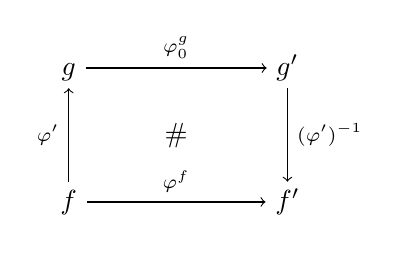
\begin{tikzpicture}[description/.style={fill=white,inner sep=2pt}]
\matrix (m) [matrix of math nodes, row sep=1em,column sep=2.5em, text height=1.5ex, text depth=0.25ex]
{ g& & g' \\
&\#&\\
  f &  &f' \\ };
\path[->](m-1-1) edge node[auto] {$\scriptstyle \varphi^g_0$}(m-1-3);
\path[->](m-3-1) edge node[auto]{$\scriptstyle \varphi^f$}(m-3-3);
\path[->](m-3-1) edge node[auto]{$\scriptstyle \varphi'$}(m-1-1);
\path[->](m-1-3) edge node[auto]{$\scriptstyle (\varphi')^{-1}$}(m-3-3);
\end{tikzpicture}.
\end{center}
According to Lemma \ref{equivalences}, $\phi^g_0(g)=g'$. Hence $\phi^f_0(f)=(\phi')^{-1}\circ\phi_0^g\circ\phi'(f)=f'$, from which the result easily follows.
\end{proof}

\begin{prop}
Considering the real cases of main type $J_{10}$, allowing only real transformations, the following equivalences are all the equivalences that hold between different subcases and different values of the parameter $a$:
\begin{itemize}
\item $ J_{10}^{-,0} \sim J_{10}^{+,\frac{3}{\sqrt{2}}}\sim J_{10}^{+,-\frac{3}{\sqrt{2}}}$;\\
\item $J_{10}^{+,a}\sim J_{10}^{+,\frac{3c_1}{\sqrt{d+3c_1^2}}}\sim J_{10}^{-,\frac{3c_2}{\sqrt{|d+3c_2^2|}}}\sim J_{10}^{+,\frac{3c_3}{\sqrt{d+3c_3^2}}}$, if $k(z)=z^3+dz+e$ has three roots $c_1<c_2<c_3$, where $e=-\frac{1}{3}a+1$ and $e=\frac{2}{27}a^3-\frac{1}{3}a$;\\
\item $J_{10}^{-,a}\sim J_{10}^{+,\frac{3c_1}{\sqrt{d+3c_1^2}}}\sim J_{10}^{-,\frac{3c_2}{\sqrt{|d+3c_2^2|}}}\sim J_{10}^{+,\frac{3c_3}{\sqrt{d+3c_3^2}}}$, if $k(z)=z^3+dz+e$ has three roots $c_1<c_2<c_3$, where $e=-\frac{1}{3}a^2-1$ and $e=\frac{2}{27}a^3+\frac{1}{3}a$.\\
\end{itemize}
(In the last case $a=\frac{3c_2}{\sqrt{|d+3c_2^2|}}$ and in the second last case $a=\frac{3c_1}{\sqrt{d+3c_1^2}}$ or $a=\frac{3c_3}{\sqrt{d+3c_3^2}}$.)
\end{prop}

\begin{proof}
Let $f=x^3+ax^2y^2\pm xy^4$ be an arbitrary polynomial of real type $J_{10}^+$ or $J_{10}^-$.  We transform $f$ to the form $f=x^3+dxy^4+ey^6$, where $d=-\frac{1}{3}a^2+1$ and $e=\frac{2}{27}a^3-\frac{1}{3}a$, if $f$ is of type $J_{10}^+$ and $d=-\frac{1}{3}a^2-1$ and $e=\frac{2}{27}a^3+\frac{1}{3}a$ if $f$ is of type $J_{10}^-$, by $x\mapsto x-\frac{a}{3}y^2$ and $y\mapsto y$. We chose a weight $w$ for the diagonal defined by $f$ with the weights of $x$ and $y$ natural numbers. 

Since  there exist a transformation $\phi'$ such that

\begin{equation}\label{phi'}
\phi'(x^3+a'x^2y^2\pm |d'|xy^4)=x^3+a''x^2y^2\pm xy^4,\quad a''=\frac{a'}{|d'|},\  a',d'\in R,
\end{equation}

it suffices to consider transformations $\phi$ such that $\phi(f)$ is of the form 
\begin{equation}\label{form}
x^3+a'x^2y^2\pm |d'|xy^4,\quad a',d'\in R.
\end{equation}
Using Proposition 6 in \cite{MS2013}, it follows that $\phi_0(x)=x$. Hence $\phi_0^w(x)=x+cy^2$ and $\phi_0^w(y)=ty$, $c,t\in\R$, $t\neq 0$. Since we only consider terms on the diagonal of $\phi(f)$, we only need to consider $\phi_0^w(f)$. Now

\begin{equation}\label{eqc}
\phi_0^w(f)=x^3+3cx^2y^2+(3c^2+t^4d)xy^4+(c^3+t^4dc+et^6)y^6.
\end{equation}

Since $c=t^2c'$, where $c'=\frac{c}{t^2}$, we rewrite (\ref{eqc}) as

\begin{equation}\label{eqc'}
\phi_0^w(f)=x^3+3t^2c'x^2y^2+t^4(3c'^2+d)xy^4+t^6(c'^3+dc'+e)y^6.
\end{equation}

Clearly, for a fixed value of $t\neq 0$, $c'$ is any value such that $c'$ is a root of $k(z)=z^3+dz+e$. Considering the transformation $\phi'$, $\phi'\circ\phi_0^w$ transform $f$ to the same polynomial, regardless the value of $t$. Hence we may assume that $t=1$ and $c=c'$. 

We consider the following cases:
\begin{itemize}
\item[(A)] $e=0$ with subcases:
\begin{itemize}
\item[(I)]$d>0$;
\item[(II)]$d<0$;
\end{itemize}
\item[(B)] $e\neq 0$ with subcases:
\begin{itemize}
\item[(I)]$k(z)$ has one real root;
\item[(II)]$k(z)$ has three real roots, with subcases:
\begin{itemize}
\item[(i)] $d\ge 0$;
\item[(ii)] $d<0$;
\end{itemize}
\end{itemize}
\end{itemize}

(A) We consider the case when $e=0$. In this case $k(z)=z^3+dz=z(z^2+d)$.

(I) If $d>0$ (i.e. $f$ is of type $J_{10}^+$) the only root of $k$ is $0$ (i.e.~$c=0$) from which it follows that $\phi$ is the identity. Clearly $\phi'$ is then also the identity and the only possible value for $a''$ in (\ref{phi'}) is $0$.

(II) If $d<0$ (i.e.~$f$ is of type $J_{10}^+$ and $a=\pm\frac{3}{\sqrt{2}}$, or $f$ is of type $J_{10}^-$ and $a=0$) then $0$, $\sqrt{|d|}$ and $-\sqrt{|d|}$ are roots of $k$ (i.e. $c=0$ or $c=\sqrt{|d|}$ or $c=-\sqrt{|d|}$). In the first case $\phi$ and $\phi'$ are both the identity. In the last two cases $3c^2=-3d>0$ which implies that $3c^2+d=-2d>0$. Considering (\ref{eqc'}) and $\phi'$, taking into account that $\frac{3\sqrt{|d|}}{\sqrt{-2d}}=\frac{3}{\sqrt{2}}$, the following equivalences are all the equivalences between $f$ and germs in the families of polynomials defining the normal forms of main case $J_{10}$:
\begin{eqnarray*}
f&\sim&x^3-xy^4;\\
f&\sim&x^3+\frac{3}{\sqrt{2}}x^2y^2+xy^4;\\
f&\sim&x^3-\frac{3}{\sqrt{2}}x^2y^2+xy^4.
\end{eqnarray*} 
 Hence in this case $f$ is of type $J_{10}^+$ and $J_{10}^-$.

(B) In this case, note that since
\begin{eqnarray*}
k(z)&=&(z-c_1)(z-c_2)(z-c_3)\\
&=&z^3-(c_1+c_2+c_3)z^2+(c_1c_2+c_1c_3+c_2c_3)z-c_1c_2c_3,
\end{eqnarray*}
it follows that
\begin{equation}\label{RelationOfRoots}
c_1+c_2+c_3=0\quad\textnormal{and}\quad c_1c_2+c_1c_3+c_2c_3=d,
\end{equation}
where $c_1$, $c_2$ and $c_3$ are the complex roots of $k$.

(I) We firstly consider the case when $k$ has one real root $c_1$ and two roots that are complex conjugates $c_2$ and $c_3$, i.e.~there is only one possible value for $c$, namely $c_1$. It follows from (\ref{RelationOfRoots}) that $c_2c_3=d+c_1^2$. Since the product of two complex conjugates are positive $d+c_1^2>0$ which implies that $d+3c_1^2>0$. This means, considering (\ref{eqc'}), that $f$ is of type $J_{10}^+$. Since there is only one possible value of $c$, there is only one possible transformation that transforms $f$ to (\ref{form}) and thus only one possible type $J_{10}^+$ and only one possible value of $a''$, namely $a$.

(II) We now consider the case where $k$ has three real roots $c_1$, $c_2$ and $c_3$. The three roots must be different, otherwise $k(z)$ and $k'(z)$ have a similar root which implies, considering (\ref{eqc'}), that $f$ is degenerate. Hence $a''$ has three different values, namely $\frac{3c_j}{\sqrt{|d+3c_j^2|}}$, $j=1,2,3$, putting $c=c_j$ respectively.

Let $c_1<c_2<c_3$. Now, since $c_1+c_2+c_3=0$ not all three roots have the same sign. Firstly we consider the case when $k$ has only one negative root, i.e.~$c_1<0$ and $c_2,c_3\ge 0$. In this case note that $|c_1|=|c_2+c_3|=|c_2|+|c_3|$, i.e.~$|c_1|>|c_2|$ and $|c_1|>|c_2|$. Then $3c_1^2+d=3c_1^2+c_1c_2+c_1c_3+c_2c_3>0$, since $|c_1^2|>|c_1c_3|$, $|c_1^2|>|c_1c_2|$ and $c_1^2>0$, while $c_1c_2<0$ and $c_1c_3<0$. Hence, putting $c=c_1$, $f$ is transformed to $J_{10}^+$.
Furthermore $3c_i^2+d=3c_j^2+c_1(c_2+c_3)+c_2c_3=3c_j^2-(c_2+c_3)(c_2+c_3)+c_2c_3=3c_j^2-(c_2^2+c_2c_3+c_3^2)$, for $j=1,2$. Therefore, since $|c_2|<|c_3|$, putting $c=c_2$ result in $J_{10}^-$ and putting $c=c_3$ result in $J_{10}^+$.

In the case that $c_1<0$, $c_2<0$ and $c_3\ge 0$ the result follows similarly. 

Hence, if $k$ has three real roots, $f$ is of type $J_{10}^+$ and $J_{10}^-$. 
\end{proof}

Considering the above proof, note that the $J_{10}^-$ normal form is redundant. Also note that although $J_{10}^+$ covers the $\mu$-constant stratum, $J_{10}^-$ does not.
\newpage

\begin{thebibliography}{99}
\bibitem[{Arnold et al.(1985)}]{AVG1985}
Arnold, V.I., Gusein-Zade, S.M., Varchenko, A.N., 1985.
Singularities of Differential Maps, Vol.~I.
Birkh\"auser, Boston.

\bibitem[{Arnold(1974)}]{A1974}
Arnold, V.I., 1974.
Normal forms of functions in neighbourhoods of degenerate critical points.
Russ. Math. Surv. 29(2), 10-50.

\bibitem[{Decker et al.(2012)}]{DGPS}
Decker, W., Greuel, G.-M., Pfister, G., Sch{\"o}nemann, H., 2012.
\newblock {\sc Singular} {3-1-6} --- {A} computer algebra system for polynomial
computations.
\newblock {http://www.singular.uni-kl.de}.

\bibitem[{Kr\"uger(1997)}]{Kruger}
Kr\"uger, K., 1997.
Klassifikation von Hyperfl\"achensingularit\"aten.
Diploma Thesis, University of Kaiserslautern.

\bibitem[{Greuel et al.(2007)}]{GLS2007}
Greuel, G.-M., Lossen, C., Shustin E., 2007.
Introduction to Singularities and Deformations.
Springer, Berlin.

\bibitem[{Greuel and Pfister(2008)}]{GP2008}
Greuel G.-M., Pfister G., 2008.
A Singular Introduction to Commutative Algebra, second ed.
Springer, Berlin.

\bibitem[{Kr\"uger(2012)}]{classify}
Kr\"uger, K., 2012.
{\tt classify.lib}. {A} {\sc Singular} {3-1-6} library for classifying isolated
hypersurface singularities w.r.t.\@ right equivalence, based on the
determinator of singularities by V.I. Arnold.

\bibitem[{Marais and Steenpa\ss(2012)}]{realclassify}
Marais, M., Steenpa\ss, A., 2012.
{\tt realclassify.lib}. {A} {\sc Singular} {3-1-6} library for classifying
isolated hypersurface singularities over the reals w.r.t.\@ right equivalence.

\bibitem[{Marais and Steenpa\ss (2013)}]{MS2013}Marais, M.S., Steenpa\ss, A., 2013.
The classification of real singularities using \textsc{Singular}. Part I: Splitting Lemma and Simple Singularities.
\bibitem[{Pfister and De Jongh (2000)}]{PdJ2000}
Pfister, G., De Jongh, T., 2000.
Local analytic Geometry, Amer. Math. Soc.

\bibitem[{Siersma(1974)}]{Siersma}
Siersma D., 1974.
Classification and Deformation of Singularities.
Dissertation, University of Amsterdam.

\bibitem[{Tobis(2012)}]{roots}
Tobis, E., 2012.
{\tt rootsur.lib}. {A} {\sc Singular} {3-1-6} library for counting the number
of real roots of a univariate polynomial.
\end{thebibliography}
\end{document}
